\documentclass[a4paper,10pt]{article}

\usepackage[brazilian]{babel}
\usepackage[utf8]{inputenc}
\usepackage{titlesec}
\usepackage{graphicx}
\usepackage{mathtools}
\usepackage{amsthm}
\usepackage{amsfonts}
\usepackage[top=1.0in,bottom=1.0in]{geometry}
\usepackage{hyperref}
\usepackage[singlelinecheck=false]{caption}
\usepackage[backend=biber,url=true,doi=true,eprint=false]{biblatex}
\usepackage{enumitem}
\usepackage[x11names, rgb]{xcolor}
\usepackage{tikz}
\usepackage{abstract}
\usepackage{indentfirst}
\usepackage[justification=centering]{caption}

\usetikzlibrary{snakes,arrows,shapes}

\addbibresource{references.bib}

\newcommand\blfootnote[1]{%
  \begingroup
  \renewcommand\thefootnote{}\footnote{#1}%
  \addtocounter{footnote}{-1}%
  \endgroup
}

\DeclareMathOperator*{\argmin}{arg\,min}
\DeclareMathOperator*{\argmax}{arg\,max}

\newcommand\defeq{\mathrel{\overset{\makebox[0pt]{\mbox{\normalfont\tiny\sffamily def}}}{=}}}

\renewcommand{\abstractnamefont}{\normalfont\Large\bfseries}

\titleformat{\section}
  {\normalfont\scshape\bfseries}{\thesection}{1em}{}
\titleformat{\subsection}
  {\normalfont\scshape\bfseries}{\thesubsection}{1em}{}
\titleformat{\paragraph}
  {\normalfont}{\theparagraph}{1em}{}
\titleformat{\subparagraph}
  {\normalfont}{\thesubparagraph}{1em}{}

\captionsetup[table]{labelsep=space}

\theoremstyle{plain}

\newtheorem*{thm-def}{Definição}
\newtheorem*{thm-thm}{Teorema}

\setlength{\parskip}{1em}

\begin{document}

\begin{titlepage}
  \begin{center}
    \LARGE
    \textbf{Jogando Atari e (S)NES com Aprendizado de Máquina e Redes Neurais}

    \vspace{1.7cm}
    \Large
    Um estudo superficial sobre automatização de jogos com aprendizado baseado em reforço e
    redes neurais artificiais

    \vspace{1.7cm}
    \Large
    Renato Lui Geh

    \vfill
    \Large
    Universidade de São Paulo

    Instituto de Matemática e Estatística

    Monografia para MAC0412
    \vspace{1.5cm}
  \end{center}
\end{titlepage}

\newpage
\null\vspace{\fill}
\begin{abstract}
  \large
  A proposta deste trabalho é apresentar os conceitos de aprendizado baseado em reforço com o uso
  de processos de decisão markovianos, redes neurais artificiais, como aplicar aprendizado em redes
  neurais, as especificações de \textit{hardware} tanto do Atari 2600 quanto do NES e finalmente
  analisar como foi aplicado aprendizado em um agente jogador automático.

  Este trabalho foi baseado no artigo da Google DeepMind \textit{Human-level control through deep
  reinforcement learning}\cite{mnih-et-al}, onde Mnih \textit{et al} explicam um novo algoritmo de
  aprendizado de Q-networks profundas que teve melhor performance em experimentos realizados no
  Atari 2600 do que outros algoritmos. O artigo \textit{The First Level of Super Mario Bros. is
  Easy with Lexicographic Ordering and Time Travel... \small{after that it gets a little tricky}}
  \cite{dr-murphy}, que explica como extrair uma função objetivo a partir da memória usada em
  plataformas NES, também teve grande influência nesta monografia.

  Nesta monografia serão primeiro apresentados os conceitos de aprendizado de máquina, processos
  de decisão markovianos, aprendizado baseado em reforço e redes neurais artificiais nesta ordem.
  Em seguida serão apresentadas as diferenças entre o método de automatização usado em Mnih
  \textit{et al} e o apresentado em \textit{Murphy}.
\end{abstract}
\vspace{\fill}
\newpage
\large
\tableofcontents
\normalsize
\newpage
\section{Introdução}

A monografia é dividida em 5 tópicos: introdução, noções fundamentais de probabilidade, processos
de decisão markovianos, aprendizado baseado em reforço, redes neurais artificiais, hardware e
finalmente automatização de um agente jogador.

Quando dizemos um agente jogador automático, queremos dizer um agente que performe de forma
racional e ótima no contexto do jogo. Um agente jogador automático ideal não é restringido por
regras específicas de um dado jogo, mas performa de forma ótima em todos os jogos. Por exemplo,
se o agente está jogando \textit{Breakout} de forma ótima, então o mesmo agente deve se comportar
de forma ótima em um outro jogo (por exemplo \textit{Montezuma's Revenge}) sem nenhuma
modificação no código.

\begin{figure}[h]
  \centering{
    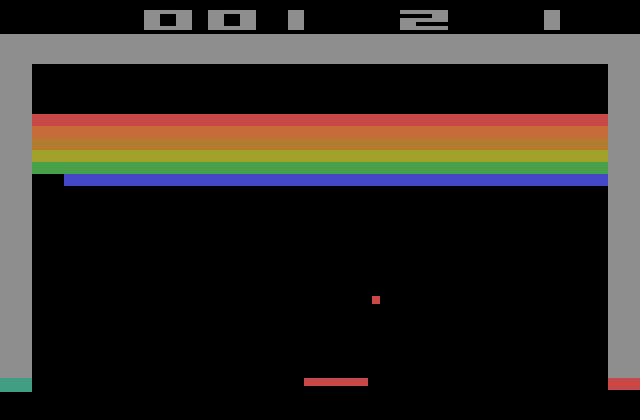
\includegraphics[scale=0.3]{imgs/breakout.png}
    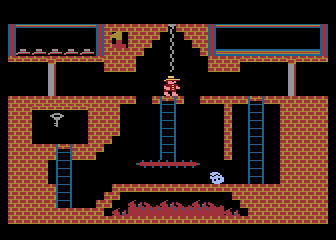
\includegraphics[scale=0.525]{imgs/montezuma.png}
    \caption{\textit{Breakout} (à esquerda) e \textit{Montezuma's Revenge} (à direita) no Atari
    2600. \textit{Fonte:} \url{http://en.wikipedia.org/} e \url{http://www.atariprotos.com/}}
  }
\end{figure}

Infelizmente, tal agente não existe ainda. De fato, Mnih \textit{et al}\cite{mnih-et-al} mostram,
por meio de experimentos, que o agente teve um desempenho impressionante em \textit{Breakout},
mas foi muito mal em \textit{Montezuma's Revenge}. Isso é dado pela variedade de controles,
objetivos e condições de recompensa que cada jogo possue. Um agente ideal conseguiria aprender
todos os elementos de um jogo tal como um jogador humano dados todos estímulos visuais do próprio
jogo. No entanto, isso implica no reconhecimento de elementos específicos da tela como o domínio
de uma função que mapeia estímulos visuais a uma recompensa (seja imediata ou a longo prazo).

Uma outra alternativa seria o uso dos bits ``crus'' do próprio jogo para determinar que um objeto
seja mapeado na função objetivo (recompensa). Esta abordagem, no entanto, não indica que o agente
está sendo ``inteligente'' \footnote{A questão de um agente ser inteligente ou não é uma questão
mais filosófica e que requer um estudo muito mais aprofundado do que o que é exposto nesta
monografia}, mas que está apenas seguindo, de forma gulosa, a melhor recompensa direta a partir
de uma função já existente.

A diferença da abordagem visual e da abordagem ``crua'' pode ser comparada a um agente aprender
vendo vários vídeos de pessoas jogando um certo jogo ou aprender lendo um manual que aponta
exatamente quais ações o jogador deve tomar para que seu desempenho seja ótimo. Enquanto que os
dois métodos consistem na maximização das ações para gerar o melhor resultado, a abordagem visual
é um método muito mais geral e semelhante a como humanos se comportam. Além disso, a abordagem
crua depende da especificação do hardware e do jogo. Nesta monografia abordaremos principalmente
pelo lado visual, já que queremos um agente que seja independente da implementação usada.

\subsection*{Noções de Probabilidade}

O uso de probabilidades na área de Inteligência Artificial não foi imediata. A princípio, o método
preferível de se representar conhecimento era por meio de lógicas. Para representarmos algo que
existisse consideraríamos algum evento como verdadeiro. Uma relação de causa-efeito é dada por uma
implicação. Por exemplo, se desejássemos representar um mundo onde todo ser que come grama é uma
cabra, e que todo ser que come carne é urso, então diríamos que nossa base de conhecimento é
composta por:

\begin{align*}
  &Cabra, \quad Urso \\
  &Grama, \quad Carne \\
  &Come(X, Y) \\
  &\forall x, Come(x, Grama) \to Cabra \\
  &\forall x, Come(x, Carne) \to Urso
\end{align*}

No entanto, é fácil notar que quanto mais seres incluírmos no nosso mundo, mais regras precisamos
criar. Além disso no mundo anterior consideramos que um ser come grama se e somente se o ser é uma
cabra, e um ser come carne se e somente se o ser é um urso. Porém, digamos que existe um ser
chamado humano que come tanto grama quanto carne. Precisamos criar regras que diferencie um urso de
um humano e um humano de uma cabra. As lógicas mais tradicionais não conseguem lidar com elementos
que se justapõem sem diferenciarmos explicitamente com regras. De fato, uma das maiores
desvantagens da lógica é a enumeração exaustiva de todas as regras.

Podemos resolver este problema por meio de probabilidades. Considere o mundo anterior e digamos que
existe uma população de 60 cabras, 30 ursos e 10 humanos neste mundo. Então podemos construir a
seguinte tabela de probabilidades condicionais:

\begin{table}[h]
  \begin{center}
    \begin{tabular}{l | c  c}
      Animal & $P(Animal=x | Come=grama)$ & $P(Animal=x | Come=carne)$ \\
      \hline
      Cabra & 0.857 & 0.00 \\
      Humano & 0.143 & 0.250 \\
      Urso & 0.00 & 0.750 \\
    \end{tabular}
  \end{center}
\end{table}

A primeira coluna categoriza um $Animal$ como uma das três possíveis opções: Cabra, Humano e Urso.
Cada $i$-ésima linha mostra a probabilidade condicional de $Animal$ ser $x$ dado que o que ele come
é grama ou carne. Note que toda coluna de probabilidades deve somar 1. Isto ocorre por que
temos conjuntos exaustivos que cobrem o nosso mundo inteiro. Para toda comida, o animal relativo
a ele deve estar contido em alguma população de animal.

Chamamos as probabilidades condicionais da forma $P(X=\{x_1,...,x_n\} | E=\{e_1,...,e_n\})$ de
probabilidades posteriores, onde $X$ é o conjunto de variáveis e $E$ é o conjunto de evidências
(variáveis observáveis do nosso mundo). As probabilidades da forma $P(X)$ são chamadas de
probabilidades \textit{a priori}.

\section{Aprendizado de Máquina}

Aprendizado de máquina pode ser visto como um jeito de aproximar uma função dados valores da função
somados a um erro. Ou seja, queremos uma função que minimize o erro dos valores dados com os
valores obtidos pela função. Por exemplo, na função dada pela Figura 2, queremos uma função que
consiga achar uma aproximação dos mesmos valores obtidos nos pontos azuis. Chamamos os pontos
azuis -- ou seja, os dados observados -- de conjunto de treino, já que iremos usar estes pontos
para treinar uma função para que ela consiga achar uma predição de menor erro possível para outros
pontos.

Em outras palavras, queremos achar uma função $f$ tal que:

\begin{equation*}
  f(x) = \argmin_{a, b} \sum_i (y_i - ax_i + b)^2
\end{equation*}

\newpage

\begin{figure}[h]
  \centering{
    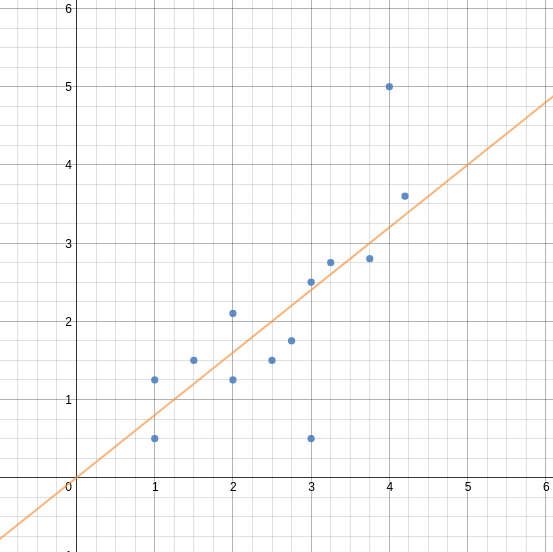
\includegraphics[scale=0.35]{imgs/learn_graph1.png}
    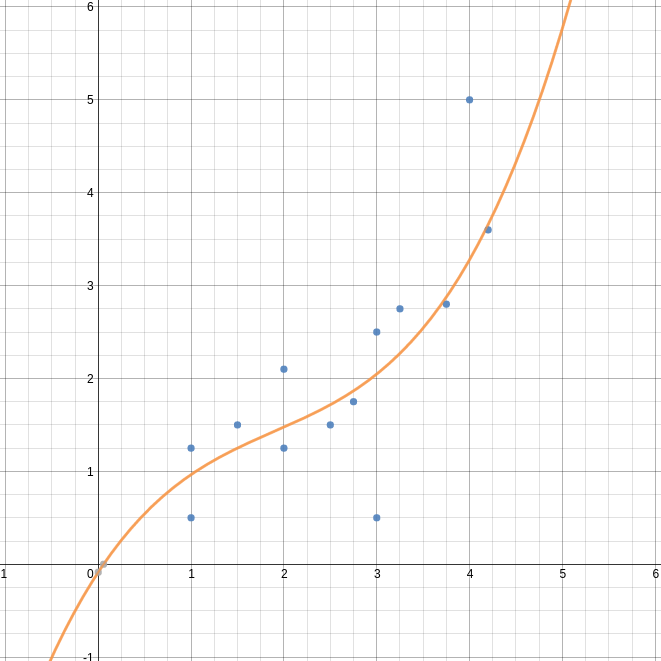
\includegraphics[scale=0.2915]{imgs/learn_graph2.png}
    \caption{Dados os valores de treino dado pelos pontos azuis no grafo, queremos uma função que
    minimize o erro $\sum_i (y_i - f(x_i))^2$ (dada pela função laranja).}
  }
\end{figure}


A partir de um conjunto de treino, podemos formular diferentes funções. Por exemplo, na Figura 2
podemos usar tanto a função à esquerda quanto à direita. Na função linear há um erro grande
entre $(5, 4)$ e $f(5)$, enquanto que na função à direita o erro é menor em $x=5$, mas o erro
é maior em outros pontos. A complexidade de uma função não depende somente do conjunto de treino,
mas também do conjunto de testes, ou seja, do conjunto que vamos tentar aproximar depois de termos
treinado a função. Um conjunto de testes que tenha valores excepcionais ou completamente diferentes
do conjunto de treino terá, obviamente, valores com alto erro. Precisamos, portanto, escolher um
conjunto de treino que, preferencialmente, cubra uma grande parte dos casos.

Se tentarmos especializar demais a função no conjunto de treino, o aprendizado sofrerá \textit{
overfitting}, ou seja, a função estará viesada demais, e provavelmente terá uma performance ruim
quando exposta a valores novos. O caso contrário, \textit{underfitting}, ocorre quando não temos
um conjunto de treino que cobre uma parte razoável dos possíveis valores.

\section{Processos de Decisão Markovianos}

Processos de Decisão Markovianos, que chamaremos de MDPs a partir de agora, são um jeito de se
representar o mundo e as decisões que impactam neste mundo. MDPs são utilizadas para demonstrar
escolhas de decisões complexas em um espaço de estado estocástico. Nesta seção iremos primeiro
definir o que uma função de utilidade significa, em seguida vamos mostrar algumas notações usadas
em MDPs, e finalmente vamos ver como achar a melhor decisão em cada estado de uma MDP.

\subsection{Função de Utilidade}

Tomemos como exemplo o mundo de João. João adora doces e decidiu ir a doceria. No entanto a doceria
possui uma grande variedade de doces, e apesar de João querer comprar todos os doces, ele possue
uma quantidade finita de dinheiro, infelizmente. Portanto, João deseja maximizar o aproveitamento
de doces limitado pela quantidade de dinheiro que ele possue.

Digamos que João gosta de caramelo, mas em qualquer situação João prefere trufa de chocolate à
caramelo. Analogamente, João prefere alfajores exclusivamente a trufas de chocolate. Mas quando
se trata de brigadeiros, João não tem preferência entre brigadeiros e trufas. Podemos representar o
mundo de João como:

\begin{align*}
  &Alfajor \succ Trufa &\text{João prefere Alfajor a Trufa.} \\
  &Brigadeiro \sim Trufa &\text{João é indiferente entre Brigadeiro e Trufa.} \\
  &Alfajor \succ Caramelo &\text{João prefere Alfajor a Caramelo por transitividade.}\\
\end{align*}

Preferenciabilidade possue seis axiomas que iremos apenas enumerar:

\begin{enumerate}
  \item Orderabilidade
  \item Transitividade
  \item Continuidade
  \item Substitutabilidade
  \item Monotonicidade
  \item Decomponibilidade
\end{enumerate}

Pode-se ler mais sobre os axiomas na subseção 16.2.1 do livro \textit{Artificial Intelligence: A
Modern Approach}\cite{aima}.

A partir dos axiomas de preferência podemos construir uma função de utilidade que representa as
preferências de um agente. De fato, a partir dos axiomas podemos construir as seguintes
consequências para funções de utilidade\footnote{A prova para estas construções podem ser lidas em
\textit{Theory of Games and Economic Behavior}\cite{neumann-morgenstern}}:

\begin{itemize}
  \item \textbf{Existência de uma função de utilidade}: Se um agente obedece os axiomas de
    utilidade então existe uma função de utilidade que $U$ tal que $U(A) > U(B)$ se e somente se
    $A \succ B$. Analogamente existe um $U$ tal que $U(A) = U(B)$ se e somente se $A \sim B$.
  \item \textbf{Utilidade esperada de uma loteria}: A utilidade de uma loteria é a soma das
    probabilidades dos possíveis resultados vezes a utilidade do resultado. Ou seja, $U(L=[p_1,S_1;
    ...;p_n,S_n]) = \sum_i p_iU(S_i)$.
\end{itemize}

Uma loteria $L$ é o conjuntod de todos os possíveis resultados que podem ocorrer com suas
respectivas probabilidades, ou seja, $L = [p_1,S_1;...;p_n,S_n]$, onde $p_1,...,p_n$ são as
probabilidades dos resultados $S_1,...,S_n$.

Podemos também chamar a utilidade esperada de uma ação $S_i$ como $EU(S_i)$. Se queremos achar a
melhor ação $a^*$ que maximize a utilidade esperada, então queremos:

\begin{equation*}
  a^* = \argmax_a EU(a|\mathbf{e})
\end{equation*}

Ou seja, queremos a melhor ação que dê uma utilidade esperada maximal dada uma evidência de
variáveis observáveis $\mathbf{e}$.

Funções de utilidade servem como uma forma de medir a preferência de uma ação em relação a outra,
e serão usadas em MDPs como uma função medidora de cada estado da MDP.

\newpage

\subsection{MDPs}

Considere que existe um robô que transita no espaço de estados mostrado na Figura 3. Cada estado
possue uma recompensa, sendo os estados terminais $(4, 3)$ e $(4, 2)$ com recompensa +1 e -1
respectivamente e em todos os outros estados recomensa -0.04.

\begin{figure}[h]
  \begin{center}
    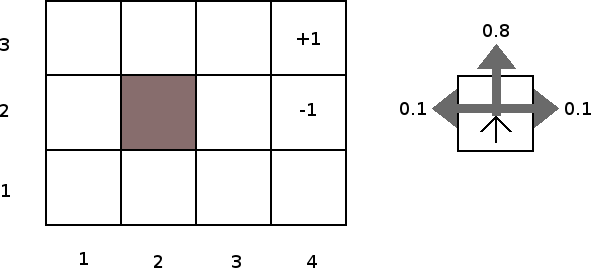
\includegraphics[scale=0.4]{imgs/grid4x3.png}
  \end{center}
  \caption{O robô começa na posição $(1, 1)$. Os estados terminais em $(4, 3)$ e $(4, 2)$ tem
  recompensas +1 e -1 respectivamente. Em todo outro estado a recompensa é de -0.04. O quadro a
  direita indica que com probabilidade 0.8 o robô consegue se movimentar na direção desejada. Com
  0.1 de probabilidade o robô movimenta-se $90^o$ a esquerda e com 0.1 $90^o$ a direita.}
\end{figure}

Se o ambiente fosse determinístico, achar o melhor caminho seria fácil, consistindo-se apenas de
uma busca pelo espaço de estados. No entanto, o robô não é confiável, já que tanto os sensores
quanto motores são longe de ideais. Isso significa que o robô, com probabilidade 0.8, consegue de
fato ir para o estado adjacente desejado, mas com probabilidade 0.2 o agente se move para qualquer
um dos dois outros estados a $90^o$ com distribuição uniforme.

Assumindo-se o ambiente como totalmente observável, então a solução para este problema se trata de
se achar a melhor ação em todos os estados, já que se ação falhar teremos uma melhor ação para o
estado seguinte.

Chamamos de modelo de transição o resultado de cada ação em cada estado. Pelo ambiente neste
problema ser estocástico, então representamos o modelo de transição como a probabilidade
$P(s'|s,a)$, ou seja, a probabilidade de se ir para um estado seguinte $s'$ dado o estado atual $s$
e a ação $a$ do agente.

No exemplo dado a recompensa pode ser vista como aditiva, pois a utilidade dos estados pode ser
representada como:

\begin{equation*}
  U([s_0,s_1,s_2,...]) = R(s_0) + R(s_1) + R(s_2) + ...
\end{equation*}

Outro jeito de se representar recompensas é por meio de recompensas descontadas:

\begin{equation*}
  U([s_0,s_1,s_2,...]) = \gamma R(s_0) + \gamma^2 R(S_1) + \gamma^3 R(S_2) + ...
\end{equation*}

O fator de desconto $\gamma$ é um número entre 0 e 1, e representa a relação entre tempo e
recompensa. Um agente que use $\gamma = 0$ não se preocupam tanto com recompensas futuras, enquanto
que quando $\gamma = 1$ o agente se preocupa com a recompensa acumulada.

Um problema que seja totalmente observável, tenha ambiente estocástico e um modelo de transição
markoviano é chamado de um processo de decisão markoviano (MDP).

\subsection{Políticas ótimas}

Chamamos de política a sequência de ações de um agente em uma MDP. Uma política ótima é aquela em
que a utilidade esperada é maximal. Ou seja, queremos uma política $\pi$ tal que:

\begin{equation*}
  U^\pi(s) = E\left[\sum_{t=0}^\infty \gamma^t R(S_t)\right]
\end{equation*}

Vamos denotar uma política ótima como $\pi^*$. Portanto:

\begin{equation*}
  \pi^*(s) = \argmax_\pi U^\pi(s) = \argmax_{a \in A(s)} \sum_{s'} P(s'|s,a)U(s')
\end{equation*}

Onde $A(s)$ é o conjunto de possíveis ações no estado $s$. Para acharmos políticas ótimas
precisamos, portanto, achar o $P(s'|s,a)U(s')$ maximal. Para isso usamos a chamada equação de
Bellman\footnote{Em homenagem a Richard Bellman (1957).}:

\begin{equation*}
  U(s) = R(s) + \gamma \max_{a \in A(s)} \sum_{s'} P(s'|s,a)U(s')
\end{equation*}

Usando a equação de Bellman no nosso exemplo do robô, temos que, no estado inicial $(1, 1)$:

\begin{align*}
  U(1, 1) = -0.04 + \gamma \max[&0.8 U(1, 2) + 0.1 U(2, 1) + 0.1 U(1, 1), &(Cima) \\
                                &0.9 U(1, 1) + 0.1 U(1, 2), &(Esquerda) \\
                                &0.9 U(1, 1) + 0.1 U(2, 1), &(Baixo) \\
                                &0.8 U(2, 1) + 0.1 U(1, 2), 0.1U(1, 1)] &(Direita)
\end{align*}

Após calcularmos as utilidades de cada estado vemos que a melhor decisão é ir para cima.

\section{Aprendizado Baseado em Reforço}

Considere uma chipanzé que daremos o nome de Lucy. Um grupo de cientistas deseja testar a
inteligência de Lucy por meio de aprendizado baseado em reforço. Para isso eles devem ter um
objetivo para Lucy: existem três botões, $A$, $B$ e $C$; o objetivo é apertar os três botões na
sequência $B$, $A$, $C$.

Vamos considerar a sequência $ABC$ como apertar os botões $A$, $B$ e $C$ nesta ordem. Esta regra
vale também para todas as outras combinações de sequência. Vamos considerar o $i$-ésimo botão como
o botão da posição $i$ na sequência. Por exemplo, o botão $i=0$ em $CAB$ é $C$, enquanto que o
botão $i=2$ em $BAC$ é $C$.

No entanto, a linguagem dos chipanzés difere radicalmente da do grupo de cientistas, e portanto
eles precisam transmitir o conhecimento de que a sequência $BAC$ é a meta através de uma linguagem
universal: bananas. Os testes de Lucy são feitos diariamente, ou seja, cada dia é um teste. Em cada
teste Lucy deve apertar alguma combinação de três botões. Porém, em cada teste, se o $i$-ésimo
botão que Lucy apertar corresponder ao $i$-ésimo botão da sequência meta, então os cientistas dão
um pedaço de banana para Lucy. Se Lucy completar a sequência completa em um teste, os cientistas
dão uma banana inteira para Lucy.

O exemplo acima ilustra o uso de aprendizado baseado em reforço. A sequência de botões corresponde
aos estados $S$, as ações de apertar o $i$-ésimo botão corresponde as ações $A(i)$ no estado $i$,
as recompensas $R(s,a)$ no estado $s$ correspondem às recompensas $R(s,a)$ e o modelo de transição
$P(s'|s,a)$ corresponde a probabilidade de Lucy ir ao próximo estado dado que ela executou a ação
$a$ de apertar um botão e dado que ela estava no estado $s$.

Podemos ver que temos as ações $A(s)$ e os estados possíveis $S$ especificados no problema, no
entanto não sabemos como nosso modelo de transição funciona. Além disso, sabíamos quanto de
recompensa dar a Lucy pois sabíamos quais passos dar para chegarmos a meta. No entanto, considere
um problema que não sabemos como chegar a meta, apenas que chegamos (neste caso Lucy apenas
receberia a recompensa quando chegasse em $BAC$). Neste caso queremos também achar $R(s,a)$.

É fácil notar que queremos achar uma MDP que tenha um modelo de transição e recompensa ideais para
chegarmos a meta de forma ótima. Portanto, o que realmente desejamos é achar uma política ótima que
nos dê a maior recompensa.

\begin{equation*}
  \pi^*(s) = \argmax_\pi U^\pi(s) = \argmax_a [R(s, a) + \gamma U^*(s')]
\end{equation*}

No entanto, não sabemos como são $R(s, a)$ e $U^*(s')$. Por isso podemos ver aprendizado por
reforço como um problema de se aprender $R(s, a) + \gamma U^*(s')$. Vamos chamar esta expressão
de $Q^*(s, a)$. Queremos, então, achar a melhor política $\pi^*$ tal que:

\begin{align*}
  &Q^*(s, a) = R(s, a) + \gamma \sum_{s'} P(s'|s,a) \max_{a'} Q^*(s', a') \\
  &\pi^*(s) = \argmax_a Q^*(s, a)
\end{align*}

Podemos criar um algoritmo que seleciona uma ação $a$ e a executa no estado $s$, recebe uma
recompensa $R(s,a)$ e em seguida atualiza $Q(s,a)$ com os novos dados encontrados. Este algoritmo
é chamado de Q-learning, e podemos fazer a atualização de $Q$ da seguinte forma:

\begin{equation*}
  Q(s, a) \gets (1-\alpha)Q(s,a) + \alpha[R(s,a) + \gamma \max_a Q(s', a')]
\end{equation*}

Onde $\alpha$ é chamada de taxa de aprendizado, e é normalmente igual a 0.1. Uma taxa de
aprendizado alta indica que o algoritmo considera mais os novos termos ao que foi visto antes. Uma
taxa baixa de aprendizado indica que o algoritmo considera mais a média de termos vistos.

\section{Redes Neurais}

A área de Inteligência Artificial sempre buscou inspirações na fisiologia humana, principalmente no
orgão que mais nos diferencia dos outros animais: o cérebro. O cérebro consiste de vários neurônios
que, interligados em conjuntos, transmitem informação através de sinapses. A ideia de Redes Neurais
é tentar imitar esta função fisiológica.

Redes Neurais são compostas por nós, ou unidades, conectadas por arestas direcionadas com pesos
associados. Cada aresta $ij$ -- ou seja, que conecta uma unidade $i$ a outra unidade $j$ -- propaga
uma ativação $a_i$ de $i$ para $j$. Além disso, o peso de cada aresta, que simboliza a força do
sinal da conexão, será denotado como $w_{ij}$. $a_0$ tem valor inicial 1.

A entrada da rede neural é dada por:

\begin{equation*}
  in_j = \sum_{i=0}^n w_{ij} a_i
\end{equation*}

Em seguida, aplica-se uma função de ativação $g$ para se derivar a saída:

\begin{equation*}
  a_j = g(in_j) = g \left(\sum_{i=0}^n w_{ij} a_i\right)
\end{equation*}

\begin{figure}[h]
  \centering {
    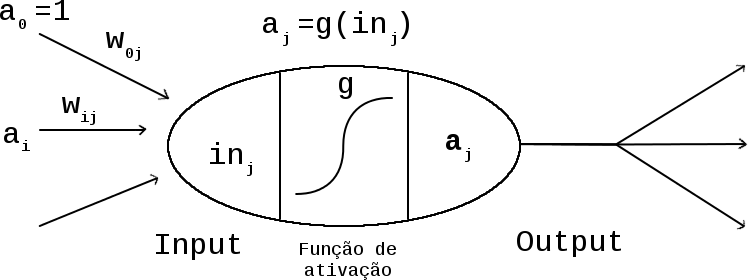
\includegraphics[scale=0.35]{imgs/neuron.png}
  }
  \caption{Um modelo para um neurônio. Ativação de saída da unidade é $a_j = g(\sum_{i=0}^n w_{ij}
    a_i)$, onde $a_i$ é a ativação da saída da unidade $i$ e $w_{ij}$ é o peso da aresta da unidade
    $i$ para esta unidade.}
\end{figure}

A função de ativação é uma função limitadora em que normalizamos a saída em um número entre 0 e 1.
Exemplos de funções de ativação são as funções \textit{hard threshold} e sigmóide, mostradas na
Figura 4. Se a rede usa uma função de \textit{hard threshold}, então a chamamos de perceptron. No
caso de uma sigmóide chamamos de um perceptron sigmóide. As duas funções de ativação garantem a
propriedade da rede neural de representar uma função não-linear. Porém, a função sigmóide tem o
benefício de ser diferenciável, enquanto que a \textit{hard threshold} não é diferenciável em 0.

\begin{figure}[h]
  \centering {
    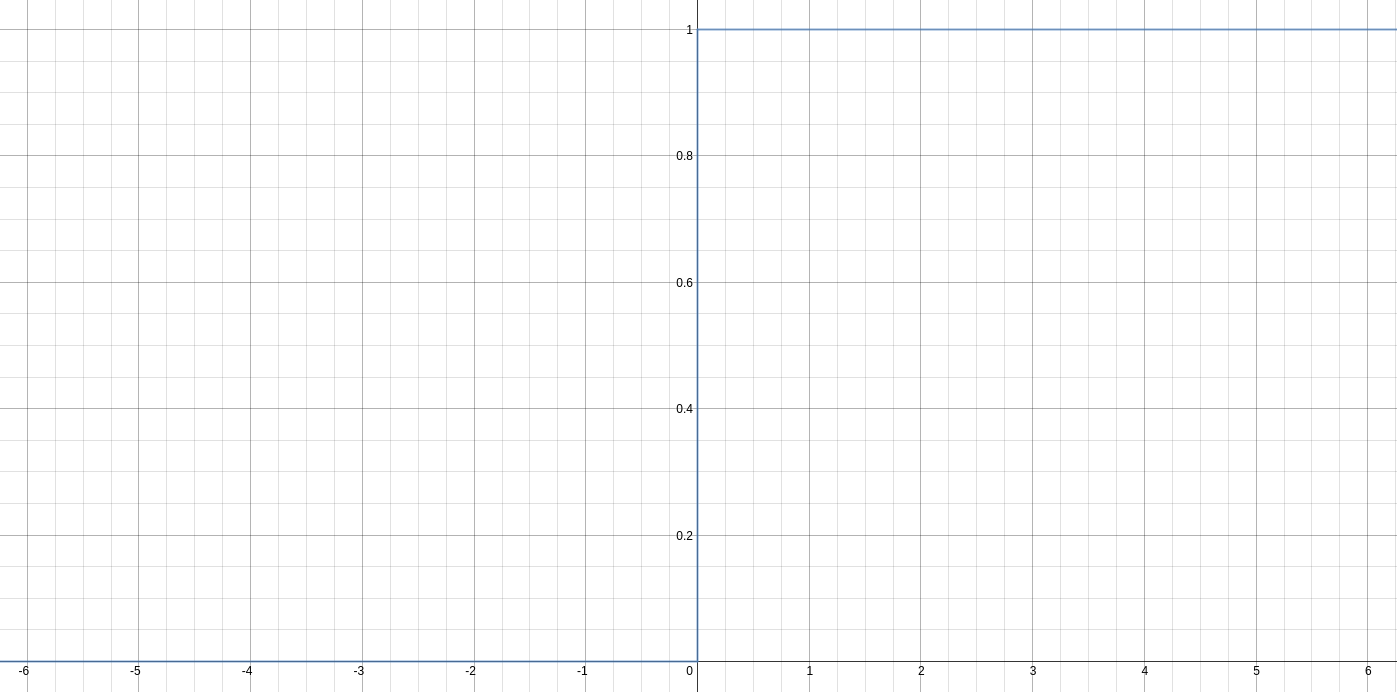
\includegraphics[scale=0.125]{imgs/hthreshold.png}
    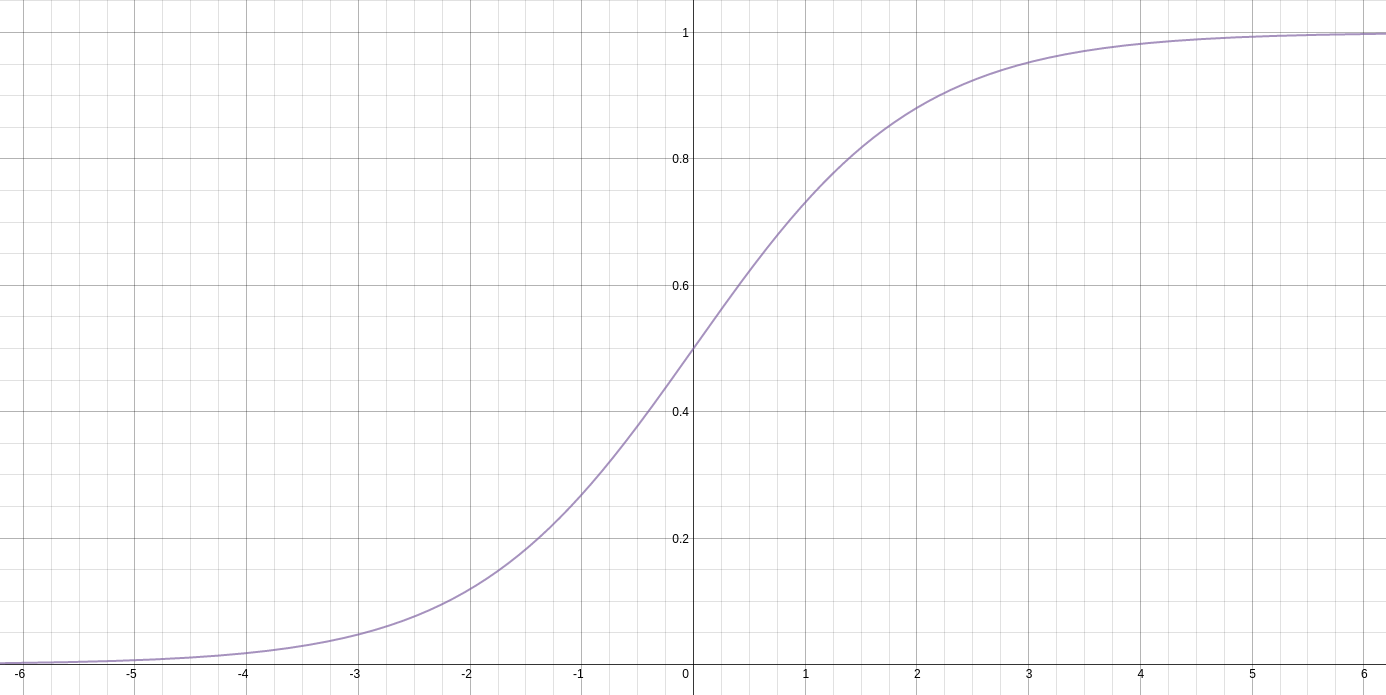
\includegraphics[scale=0.125]{imgs/sigmoid.png}
  }
  \caption{À esquerda a função \textit{hard threshold} com saída 0/1. À direita a função sigmoide
    $\frac{1}{1+e^{-z}}$.}
\end{figure}

Redes neurais são divididas em camadas. Visualizando as camadas em um espaço unidimensional como
uma reta, poderíamos dizer que as unidades mais ``à direita'' são os neurônios de saída. Cada
unidade de saída representa uma classe de saída. Para variáveis discretas, se tivermos $n$
possíveis soluções, teremos $n$ diferentes unidades representando cada solução. No caso de
variáveis contínuas podemos representar a função resultante como uma função linear por partes, com
cada função linear como solução. ``À esquerda'' temos as unidades de entrada, que corresponderão
ao primeiro estímulo da rede ao conjunto de treino. Entre as unidades de entrada e de saída podemos
ter várias outras camadas chamadas de camadas ocultas.

Aprendizado em redes neurais depende de sua função de ativação. Podemos usar a regra de aprendizado
de perceptron ou gradient descent para regressão.

\section{Hardware}

Nesta seção veremos as especificações de hardware do Atari 2600 e do Nintendo Entertainment System
(NES).

\subsection{Atari 2600}

O Atari 2600 é uma plataforma de jogos criada em 1977 pela Atari Inc., e era baseado na tecnologia
MOS 6507, um microprocessador 8-bits que possuía 8 KB de memória. O microprocessador possuía 28
pinos para configuração, com 13 pinos para endereçamento de memória e 8 para instruções. Os 7 pinos
restantes eram usados para energia, ciclos de clock, reset e controle de escrita e leitura do CPU.

O microprocessador operava em 1.19 MHz, com 128 bytes de RAM. A paleta de cores em formatos NTSC
era de 128 cores, enquanto que em formatos PAL o Atari 2600 operava em 104 cores. Vamos considerar
nesta monografia que a paleta de cores utilizada possue 128 cores. A tela era composta de 210
$\times$ 160 pixels. Além disso, devido a limitações de memória, o Atari 2600 limitava q quantidade
de artefatos mostrados na tela, separando cada objeto em dois conjuntos: par e ímpar. A cada frame,
um dos conjuntos era impresso na tela enquanto que o outro era suprimido. No frame seguinte os
conjuntos eram invertidos.

Por causa disso, em Mnih \textit{et al}\cite{mnih-et-al}, simplifica-se a tela para que a
complexidade computacional não fique demasiadamente grande.

\subsection{Nintendo Entertainment System (NES)}

O NES é baseado em um microprocessador de 8-bit rodando a 1.79Hz. Criado em 1983, ele possuía 2 KB
de RAM, com uma paleta de cores de 48 cores e 6 tons de cinza. A resolução padrão do NES é de 256
$\times$ 240 pixels. Possuía 16 pinos para configuração, com um extensor de 15 pinos.

Na memória do NES, haviam endereços específicos para atributos como vida do jogador, coordenadas na
tela e quantas tentativas restantes o jogador possuía até que o jogo declarasse que o jogador
perdeu. Por exemplo, em Super Mario Bros. o byte \texttt{0x757} contém o número de vidas do
jogador, o byte \texttt{0x75F} contém o mundo atual e \texttt{0x760} mostra o nível atual. O NES
rodava a 60 frames por segundo.

Em \textit{The First Level of Super Mario Bros. is Easy with Lexicographic Orderings and Time
Travel...\small after that it gets a little tricky}, Murphy utiliza esses endereços para determinar
se o jogador está ganhando, construindo uma função objetivo que devemos maximizar.

\section{Automatização de um Agente Jogador}

Nesta seção veremos duas maneiras de se construir um agente jogador automático.

Na primeira subseção vamos ver como Mnih \textit{et al} criaram um jogar automático para Atari 2600
onde a forma que o agente joga depende de experiências anteriores, sendo uma aplicação de
aprendizado de máquina.

Na segunda subseção veremos como usar uma função objetivo extraída a partir do hardware de um
Nintendo Entertainment System para se criar um jogador automático que joga a partir de um algoritmo
guloso que tenta maximizar a recompensa dada pelos bits que representam os pontos.

\subsection{Um agente jogador em Atari 2600}

Esta subseção se baseia nos estudos publicados em \textit{Playing Atari with Deep Reinforcement
Learning}\cite{dqn}.

Vamos definir que um ambiente $\mathcal{E}$ é um jogo de Atari sendo jogado pelo agente. Além
disso, podemos dizer que existe um conjunto de ações legais possíveis $\mathcal{A}$ que o agente
deve escolher no time-step $t$. Chamamos uma ação legal no time-step $t$ como $a_t$. Vamos
considerar que $\mathcal{E}$ é estocástico. A cada time-step, o agente observa uma imagem $x_t \in
\mathbb{R}^d$, que é representado como um vetor de pixels da tela no instante $t$. Adicionalmente
o agente recebe uma recompensa $r_t$ que significa a diferença da pontuação do jogo.

O ambiente é parcialmente observável pois o agente apenas observa imagens da tela atual. Portanto
vamos considerar as sequências de ações e observações como o vetor $s_t=[x_1,a_1,...,a_{t-1},x_t]$
e tentarmos aprendermos estratégias a partir destas sequências. Podemos considerar que todas as
sequências do jogo terminam após um número finito de time-steps, o que nos permite definir o
problema como uma MDP finita em que cada sequência é um estado distinto. A partir disso podemos
considerar a automatização do agente como um aprendizado baseado em reforço na MDP.

Vamos considerar que as recompensas tem desconto $\gamma$ por time-step. Ou seja:

\begin{equation*}
  R_t = \sum_{t'=t}^T \gamma^{t'-t}r_{t'}
\end{equation*}

Onde $T$ é o time-step final do jogo. Assim, determinamos que a função ótima $Q^*$ é dada por:

\begin{equation*}
  Q^*(s,a) = \max_\pi E[R_t|s_t=s, a_t=a, \pi]
\end{equation*}

Onde $\pi$ é a política que mapeia sequências a ações. Usando a equação de Bellman vista na seção
sobre MDPs, temos que:

\begin{equation*}
  Q^*(s,a) = E_{s' \sim \mathcal{E}} \left[r+\gamma\max_{a'}Q^*(s',a')|s,a\right]
\end{equation*}

A estratégia ótima é selecionar a ação $a'$ a fim de maximizar o valor esperado de $r+\gamma Q^*(s,
a')$. Podemos então usar a equação de Bellman para achar uma política ótima iterando pelos valores
de $Q_i$ até convergirmos. No entanto, esta solução é imprática pois estimamos cada função $Q$
separadamente para cada sequência. Portanto precisamos usar uma função de aproximação que estime
$Q(s,a;\theta) \approx Q^*(s,a)$, como uma rede neural. Dizemos uma função de rede neural
aproximadora com pesos $\theta$ uma Q-network. Podemos treinar uma Q-network minimalizando a
sequência de funções perdas $L_i(\theta_i)$:

\begin{equation*}
  L_i(\theta_i) = E_{s,a \sim \rho(\cdot)} \left[(y_i - Q(s,a;\theta_i))^2\right]
\end{equation*}

Onde $y_i = E_{s' \sim \mathcal{E}} [r+\gamma\max_{a'}Q(s',a';\theta_{i-1})|s,a]$ é o objetivo da
iteração $i$ e $\rho(s, a)$ é a distribuição de probabilidade sobre as sequências $s$ e ações $a$
e será chamada de distribuição de comportamento.

A partir disso podemos tomar o gradiente de $L_i(\theta_i)$ diferenciando com respeito aos pesos
$\theta_i$ e aplicarmos gradient descent estocástico para acharmos um máximo local que corresponda
à uma política ótima local.

A partir disso podemos construir um jogador automático. Os experimentos efetuados por Mnih \textit{
et al} podem ser vistos em:
\url{http://home.uchicago.edu/~arij/journalclub/papers/2015\_Mnih\_et\_al.pdf}.

\subsection{Um agente jogador em NES}

A abordagem usada por T. Murphy em \cite{dr-murphy} é usar os bytes da memória do NES para decidir
se o jogador está ganhando. Por exemplo, no caso de Super Mario Bros., começa-se o jogo em \texttt{
World 1-1} e em seguida \texttt{World 1-2}. Então podemos visualizar um agente que sempre quer que
nós ``aumentemos'' o valor do mundo. No entanto, após \texttt{World 1-4}, temos \texttt{World
2-1}. Portanto, considerarmos apenas os números contidos na memória não é o bastante. T. Murphy
sugere usar uma ordem lexicográfica, tornando \texttt{World 2-1} $>$ \texttt{World 1-4}. Portanto,
podemos considerar um par lexicográfico $\langle w, l \rangle$ tal que:

\begin{equation*}
  \langle w_1, l_1 \rangle < \langle w_2, l_2 \rangle
\end{equation*}

Se $w_1=w_2$ e $l_1<l_2$ ou se $w_1<w_2$ seja qual for os valores de $l_1$ e $l_2$. Deste jeito
podemos usar combinações aparentemente desconexas e junta-las de forma racional, por exemplo:
$\langle$mundo, nível, posição no eixo $x\rangle$.

A partir disso, podemos construir uma função objetivo que monitora a memória de um objetivo (por
exemplo a vida do jogador). Tomando em conta várias funções objetivos, podemos construir um jogador
automático.

Para construir estas funções objetivos, é preciso treinar o agente. Com um conjunto de treino que
corresponde a um jogador, o agente deve monitorar as várias mudanças na memória e em seguida criar
uma função objetivo para cada endereço de memória. Como foi visto na seção de Aprendizado de
Máquina, podemos criar uma função que aproxima estas mudanças. A função resultante é a função
objetivo $L_i$ para o endereço da memória $M_i$.

Para reduzir a aleatoriedade do processo de aprendizado, designa-se um peso para cada função
objetivo. Uma função objetivo ideal toma o mínimo valor no primeiro frame e o maximal no último
frame, já que queremos ordenar lexicograficamente a fim de ``avançarmos'' no jogo.

Após atribuirmos pesos às funções objetivo aprendidas, faz-se uma busca pela melhor política que
maximiza as funções objetivo.

Os experimentos efetuados por T. Murphy pode ser isto em:
\url{http://www.cs.cmu.edu/~tom7/mario/mario.pdf}.

\section{Comparação}

Nesta seção comparamos os dois métodos de aprendizado para a criação de um jogador automatizado.



\newpage
\printbibliography

\end{document}
